\begin{figure*}[t]
    \centering
    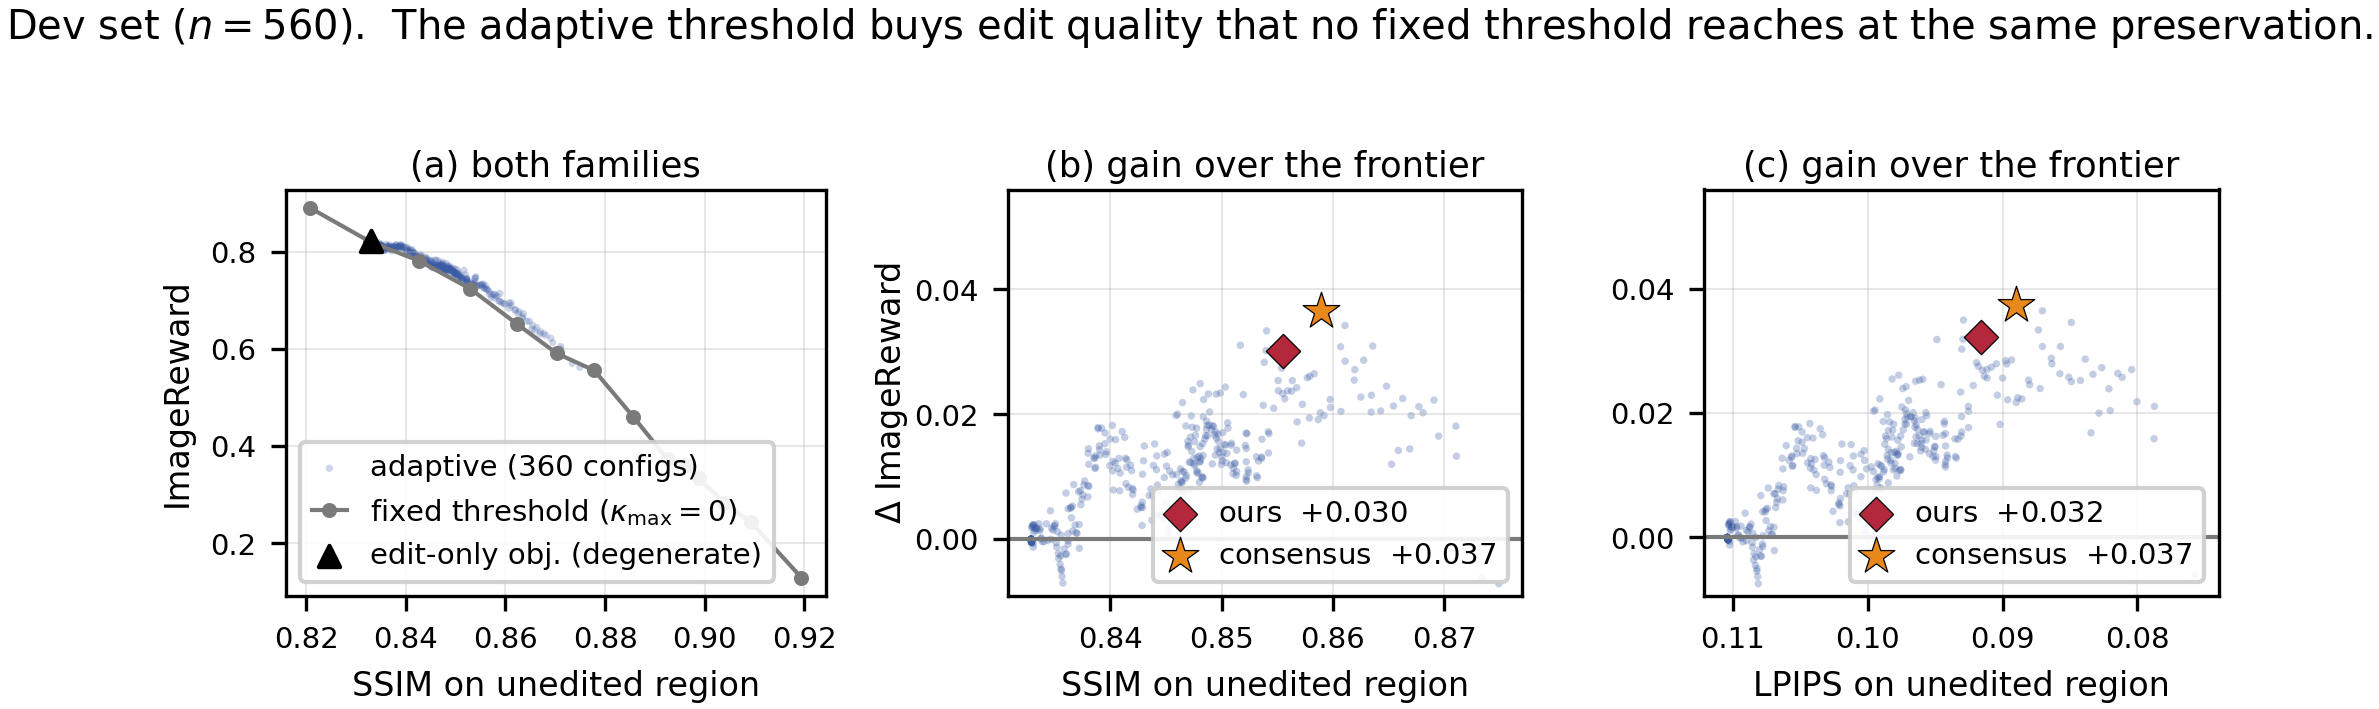
\includegraphics[width=\textwidth]{imgs/fig_adaptive_frontier.png}
    \caption{The adaptive term shifts the frontier outward. \textbf{(a)} The 360 grid configurations of the adaptive threshold against the 14 fixed levels; at this scale the two families are hard to separate, which is why (b) and (c) plot the quantity actually claimed. \textbf{(b, c)} ImageReward of each configuration minus the fixed-threshold frontier \emph{interpolated at the same preservation level}. Positive values are edit quality that no fixed threshold reaches at that preservation. The gain is consistent under two independent preservation metrics: $+0.030$ (SSIM) and $+0.032$ (LPIPS) for the parameters used in this paper, $+0.037$ for the leave-one-category-out consensus. The degenerate edit-only optimum sits on the fixed frontier by construction.}
    \label{fig:adaptive_frontier}
\end{figure*}
